\section*{Приложение А}
\addcontentsline{toc}{section}{Приложение А}
\label{sec:Appendix_1} \index{Appendix_1}
\large

\begin{figure}[ht]
\centering 
    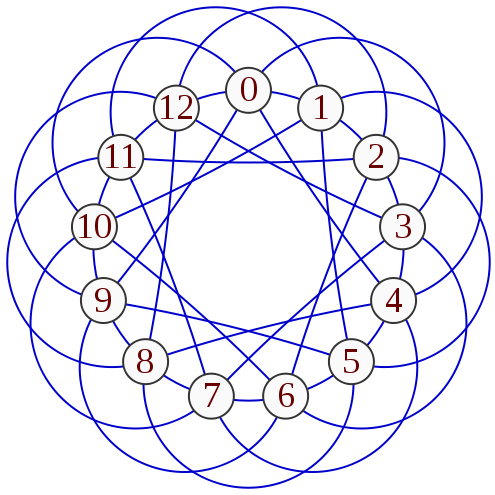
\includegraphics[scale=0.7]{image/srg_example.png}
    \caption{Граф Пейли 13-го порядка, сильно регулярный граф с параметрами srg(13,6,2,3).}
    \label{srg}
\end{figure}

\begin{figure}[H]
\centering
    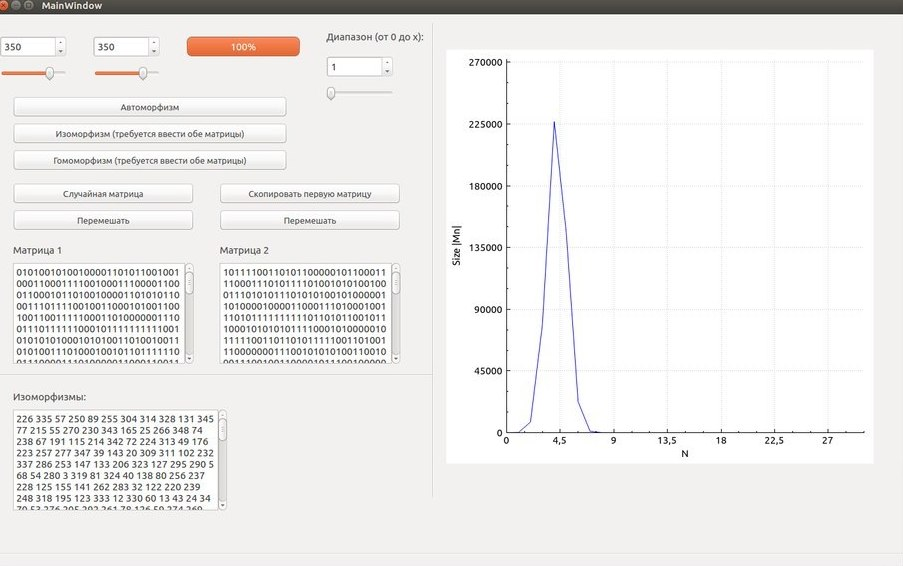
\includegraphics[scale=0.5]{image/program_example.jpeg}
    \caption{Примеры использования программы}
    \label{program_example}
\end{figure}
